\documentclass[aspectratio=43, 10pt]{beamer} % 169.

% Idioma y codificación:
\usepackage[spanish]{babel}
\usepackage[utf8]{inputenc}

% Formato de página y diseño:
\usepackage{geometry}
\usepackage{fancyhdr}
\usepackage{parskip}
\usepackage{emptypage}

% Matemática:
\usepackage{amsmath}
\usepackage{amssymb}
\usepackage{amsthm}
\usepackage{dsfont}

% Figuras:
\usepackage{graphicx}
\usepackage[labelfont=bf]{caption}

% Bibliografía y enlaces:
\usepackage[style=alphabetic]{biblatex}
\usepackage{csquotes}
\usepackage{hyperref}

% Algoritmos:
\usepackage{algorithm}
\usepackage{algpseudocode}

% Temporal:
\usepackage{xcolor}
% Operadores matemáticos:
\DeclareMathOperator*{\argmin}{arg\,min}
\DeclareMathOperator*{\argmax}{arg\,max}
\DeclareMathOperator*{\essinf}{ess\,inf}

% Conjuntos y espacios:
\newcommand{\R}{\mathbb{R}}
\newcommand{\N}{\mathbb{N}}
\newcommand{\xspace}{\mathcal{X}}
\newcommand{\yspace}{\mathcal{Y}}
\newcommand{\salgebra}{\mathcal{S}}
\newcommand{\borel}[1]{\mathcal{B}\parent{#1}}
\newcommand{\matrixspace}[2]{\mathcal{M}_{#1}\parent{#2}}
\newcommand{\power}[1]{\mathcal{P}\parent{#1}}
\newcommand{\supp}[1]{\operatorname{Supp}\parent{#1}}
\newcommand{\lspace}[2]{\operatorname{L}^{#1}\parent{#2}}
\newcommand{\continuous}[1]{\mathcal{C}\parent{#1}}
\newcommand{\continuousb}[1]{\mathcal{C}_b\parent{#1}}
\newcommand{\posmeasure}[1]{\mathcal{M}_+\parent{#1}}
\newcommand{\probmeasure}[1]{\mathcal{M}_+^1\parent{#1}}
\newcommand{\probmeasurep}[1]{\mathcal{M}_+^{1,p}\parent{#1}}
\newcommand{\cone}[1]{\R^{#1}_{++}/_\sim}

% Funciones y operadores:
\newcommand{\parent}[1]{\left(#1\right)}
\newcommand{\rparent}[1]{\left[#1\right]}
\newcommand{\norm}[1]{\left\lVert #1 \right\rVert}
\newcommand{\dotproduct}[2]{\left\langle #1,\,#2\right\rangle}
\newcommand{\trace}[1]{\operatorname{Tr}\parent{#1}}
\newcommand{\diag}[1]{\operatorname{diag}\parent{#1}}
\newcommand{\score}[2]{\nabla_{#1} \log #2}
\newcommand{\identity}[1]{\operatorname{I}_{#1}}
\newcommand{\1}{\mathds{1}}
\newcommand{\wasserstein}[2]{\mathcal{W}_{#1}\parent{#2}}
\newcommand{\weak}{\rightharpoonup}
\newcommand{\hmetric}[2]{d_{\mathcal{H}}\parent{#1,#2}}
\renewcommand{\d}{\,\operatorname{d}\!}

% Probabilidades:
\newcommand{\E}[2]{\mathbb{E}_{#1}\rparent{#2}}
\newcommand{\var}[1]{\operatorname{Var}\parent{#1}}
\newcommand{\cov}[2]{\operatorname{Cov}\parent{#1,\,#2}}
\newcommand{\ley}[1]{\operatorname{Ley}\parent{#1}}
\newcommand{\gaussian}[2]{\mathcal{N}\parent{#1,\,#2}}

% Teoría de la información:
\newcommand{\KL}[2]{\operatorname{D_{KL}}\parent{#1\,\|\,#2}}
\newcommand{\fdiv}[2]{\operatorname{D}_f\parent{#1\,\|\,#2}}
\newcommand{\TV}[2]{\operatorname{D_{TV}}\parent{#1\,\|\,#2}}
\newcommand{\DF}[2]{\operatorname{D_F}\parent{#1\,\|\,#2}}
\newcommand{\entropy}[1]{\mathcal{H}\parent{#1}}
\newcommand{\elbo}{\operatorname{ELBO}}

% Otros:
\newcommand{\feasible}[2]{\genfrac {}{}{0pt}{2}{#1}{#2}}
\newcommand{\cte}{\operatorname{constante}}
\newcommand{\gibbs}{\mathcal{K}}
\newcommand{\ptrue}{p_{\operatorname{data}}}
\newcommand{\pprior}{p_{\operatorname{prior}}}

% Imágenes:
\newcommand{\insertimage}[3]{
    \begin{figure}
        \centering
        \includegraphics[width=#2\textwidth]{./images/#1}
        \caption{#3}
        \label{fig:#1}
    \end{figure}
}

% Temporal:
\newcommand{\pendiente}[1]{\colorbox{yellow}{#1}}

\title{El Problema del Puente de Schrödinger como Generalización de los Modelos de Difusión}
\author{Fernando Fêtis Riquelme}
\institute{
    Facultad de Ciencias Físicas y Matemáticas\\
    Universidad de Chile
}
\date{Otoño, 2025}
\titlegraphic{\hfill
\includegraphics[height=1.2cm]{images/fcfm}}

\begin{document}

\frame{\titlepage}

\begin{frame}{Tabla de contenidos}
    \setbeamertemplate{section in toc}[sections numbered]
    \tableofcontents[hideallsubsections]
\end{frame}

\begin{frame}{Taxonomía de los modelos gráficos}
    \centering
    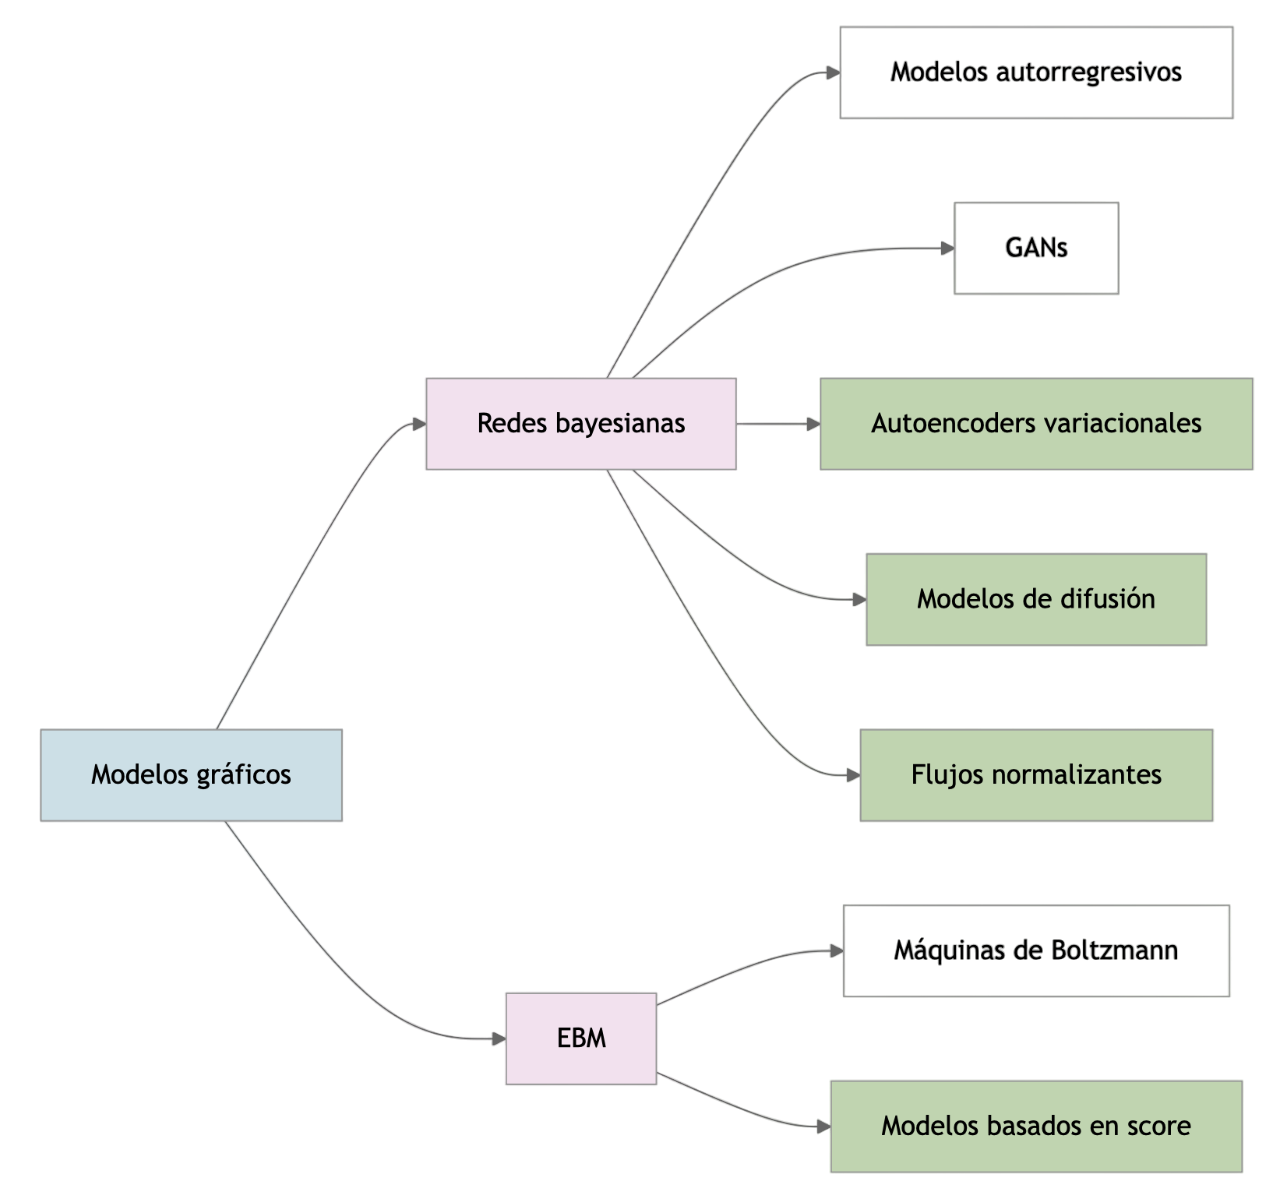
\includegraphics[width=0.7\textwidth]{images/dm/graphical_models.png}
\end{frame}

\section{Modelos de difusión}

\begin{frame}{Modelos de difusión | Diagrama general}
    \insertimage{dm/dm_diagram}{1}{Imagen obtenida desde \cite{luo2022understanding}.}
\end{frame}

\begin{frame}{Modelos de difusión | Proceso forward}
    \uncover<1->{
        El proceso de inyección de ruido es una cadena de Markov en $\R^d$ factorizada de forma causal, cuyos hiperparámetros corresponden a una secuencia finita y decreciente $(\alpha_t)_{t=1}^T\subset(0,1)$:
        \begin{block}{Proceso forward}
            \begin{equation*}
                q(x_{0:T}) = q(x_0)\prod_{t=1}^{T} q(x_t|x_{t-1}),
            \end{equation*}
            con $q(x_0) = \ptrue(x_0)$ y transiciones gaussianas isotrópicas:
            \begin{equation*}
                q(x_t|x_{t-1}) \sim \gaussian{\sqrt{\alpha_t} x_{t-1}}{(1-\alpha_t)\identity{d}}.
            \end{equation*}
        \end{block}
    }
    \uncover<2>{
        La secuencia $(\alpha_t)_{t=1}^T$ debe ser tal que
        \begin{equation*}
            q(x_T)=\int_{\parent{\R^d}^T} q(x_{0:T}) \d x_{0:(T-1)} \approx \pprior(x_T)\sim\gaussian{0}{\identity{d}}.
        \end{equation*}
    }
\end{frame}

\begin{frame}{Modelos de difusión | Proceso backward}
    \uncover<1->{
        El proceso de reconstrucción es otra cadena de Markov factorizada de forma anticausal:
        \begin{block}{Proceso backward}
            \begin{equation*}
                p_\theta(x_{0:T}) = p(x_T)\prod_{t=1}^{T} p_\theta(x_{t-1}|x_t),
            \end{equation*}
            con $p(x_T) = \pprior(x_T)$ y transiciones gaussianas:
            \begin{equation*}
                p_\theta(x_{t-1}|x_t)\sim\gaussian{\mu_\theta(x_t,t)}{\Sigma_\theta(x_t,t)}.
            \end{equation*}
        \end{block}
    }
    \begin{itemize}
        \item<2> La función de costo buscará que $p_\theta(x_{t-1}|x_t) \approx q(x_{t-1}|x_t,x_0)$.
        \item<3> Dado que $q(x_{t-1}|x_t,x_0) \sim \gaussian{\mu_q(x_0,x_t,t)}{\sigma_q^2(t)\identity{d}}$, se puede fijar $\Sigma_\theta(x_t,t)=\sigma_q^2(t)\identity{d}$.
        \item<4> Con esto, solo se necesitará aprender el vector de medias de $p_\theta(x_{t-1}|x_t)$ mediante una red neuronal $\mu_\theta:\R^d\times\{0,\ldots,T\}\to\R^d$.
    \end{itemize}
\end{frame}

\begin{frame}{Modelos de difusión | Entrenamiento e inferencia}
    \uncover<1>{
        Para entrenar $\mu_\theta$, la verosimilitud $p_\theta(x_0)=\int_{\parent{\R^d}^T} p_\theta(x_{0:T}) \d x_{1:T}$ no es tratable. En cambio, se maximiza $\E{x_0\sim \ptrue(x_0)}{\elbo(x_0)}$, donde
        \begin{equation*}
            \elbo(x_0) := \log p_\theta(x_0) - \KL{q(x_{1:T}|x_0)}{p_\theta(x_{1:T}|x_0)}.
        \end{equation*}
    }

    \uncover<2>{
        La ELBO se puede evaluar eficientemente:
        \begin{block}{ELBO para DDPM}
            Dada una muestra $x_0\sim\ptrue(x_0)$, entonces:
            \begin{equation*}
                \elbo(x_0) = -\sum_{t=1}^T \frac{1}{2\sigma_q^2(t)} \norm{\mu_q(x_0,x_t, t)-\mu_\theta(x_t,t)}^2 + \cte.
            \end{equation*}
        \end{block}
    }
    \uncover<3->{
        Para la generación de nuevas muestras desde $p_\theta(x_0)$, se simula el proceso backward comenzando con una muestra $x_T\sim\pprior(x_T)$.
    }
\end{frame}

\begin{frame}{Modelos de difusión | Formulación basada en score}
    \uncover<1->{
        Considerando que
        \begin{equation*}
            \mu_q(x_0,x_t,t) = \frac{1}{\sqrt{\alpha_t}}x_t - \frac{1-\alpha_t}{\sqrt{\alpha_t}} \fcolor{\score{x_t}{q(x_t)}},
        \end{equation*}
        la red neuronal $\mu_\theta(x_t,t)$ puede ser reparametrizada por otra red neuronal $s_\theta(x_t,t)$ que aprenda directamente $\score{x_t}{q(x_t)}$.
    }
    \begin{itemize}
        \item<2> Esto conecta los modelos de difusión con SM y con EBM.
        \item<3> Entrega un método de generación condicional (guidance):
              \begin{equation*}
                  \underbrace{\score{x_t}{p_\theta(x_t|y)}}_{\text{score condicional}} = \underbrace{\score{x_t}{p_\theta(y|x_t)}}_{\text{modelo discriminativo}} - \underbrace{\score{x_t}{p_\theta(x_t)}}_{\text{score incondicional}},
              \end{equation*}
              con $p_\theta(y|x_t)$ un clasificador o un modelo tipo CLIP.
    \end{itemize}
\end{frame}

\begin{frame}{Modelos de difusión | Formulación continua}
    La formulación basada en score permite extender los modelos de difusión a tiempo continuo usando SDEs:
    \insertimage{dm/score_sde.png}{1}{Imagen obtenida desde \cite{song2021scorebased}.}
    La función de costo se puede extender de forma \textit{natural}, obteniendo una expresión análoga a la ELBO en tiempo discreto.
\end{frame}

\begin{frame}{Modelos de difusión | Formulación continua}
    \begin{itemize}
        \item<1> DDPM y DSM son discretizaciones de SDEs específicas.
        \only<1>
        {
            \begin{equation*}
                \begin{cases}
                    \d x_t = \frac{1}{2}(1-\alpha(t))x_t \d t + \sqrt{1-\alpha(t)}\d w_t & \text{(DDPM)}\\
                    \d x_t = \sqrt{\frac{\d}{\d t}\sigma^2(t)}\d w_t & \text{(DSM)}
                \end{cases}
            \end{equation*}
        }
        \item<2> Se pueden usar diferentes solvers para el proceso backward durante la generación.
        \item<3> Existe un proceso determinista con las mismas distribuciones marginales que los procesos de difusión y denoising.
              \only<3>{\insertimage{dm/score_prob_flow.png}{0.9}{Imagen obtenida desde \cite{song2021scorebased}.}}
        \item<4> En particular, se puede calcular la verosimilitud de forma exacta.
    \end{itemize}
\end{frame}

\begin{frame}{Modelos de difusión | Limitaciones}
    \begin{itemize}
        \item<1> Sensibilidad a la elección del proceso de difusión.
        \item<2> No permite transformación entre distribuciones.
        \item<3> Convergencia asintótica a $\pprior$ y generación lenta.
    \end{itemize}
    \only<1>{
        \begin{figure}
            
\includegraphics[width=0.8\textwidth]{images/dm/linear_cosine_scheduler}
            $ $\vspace{0.3cm}
            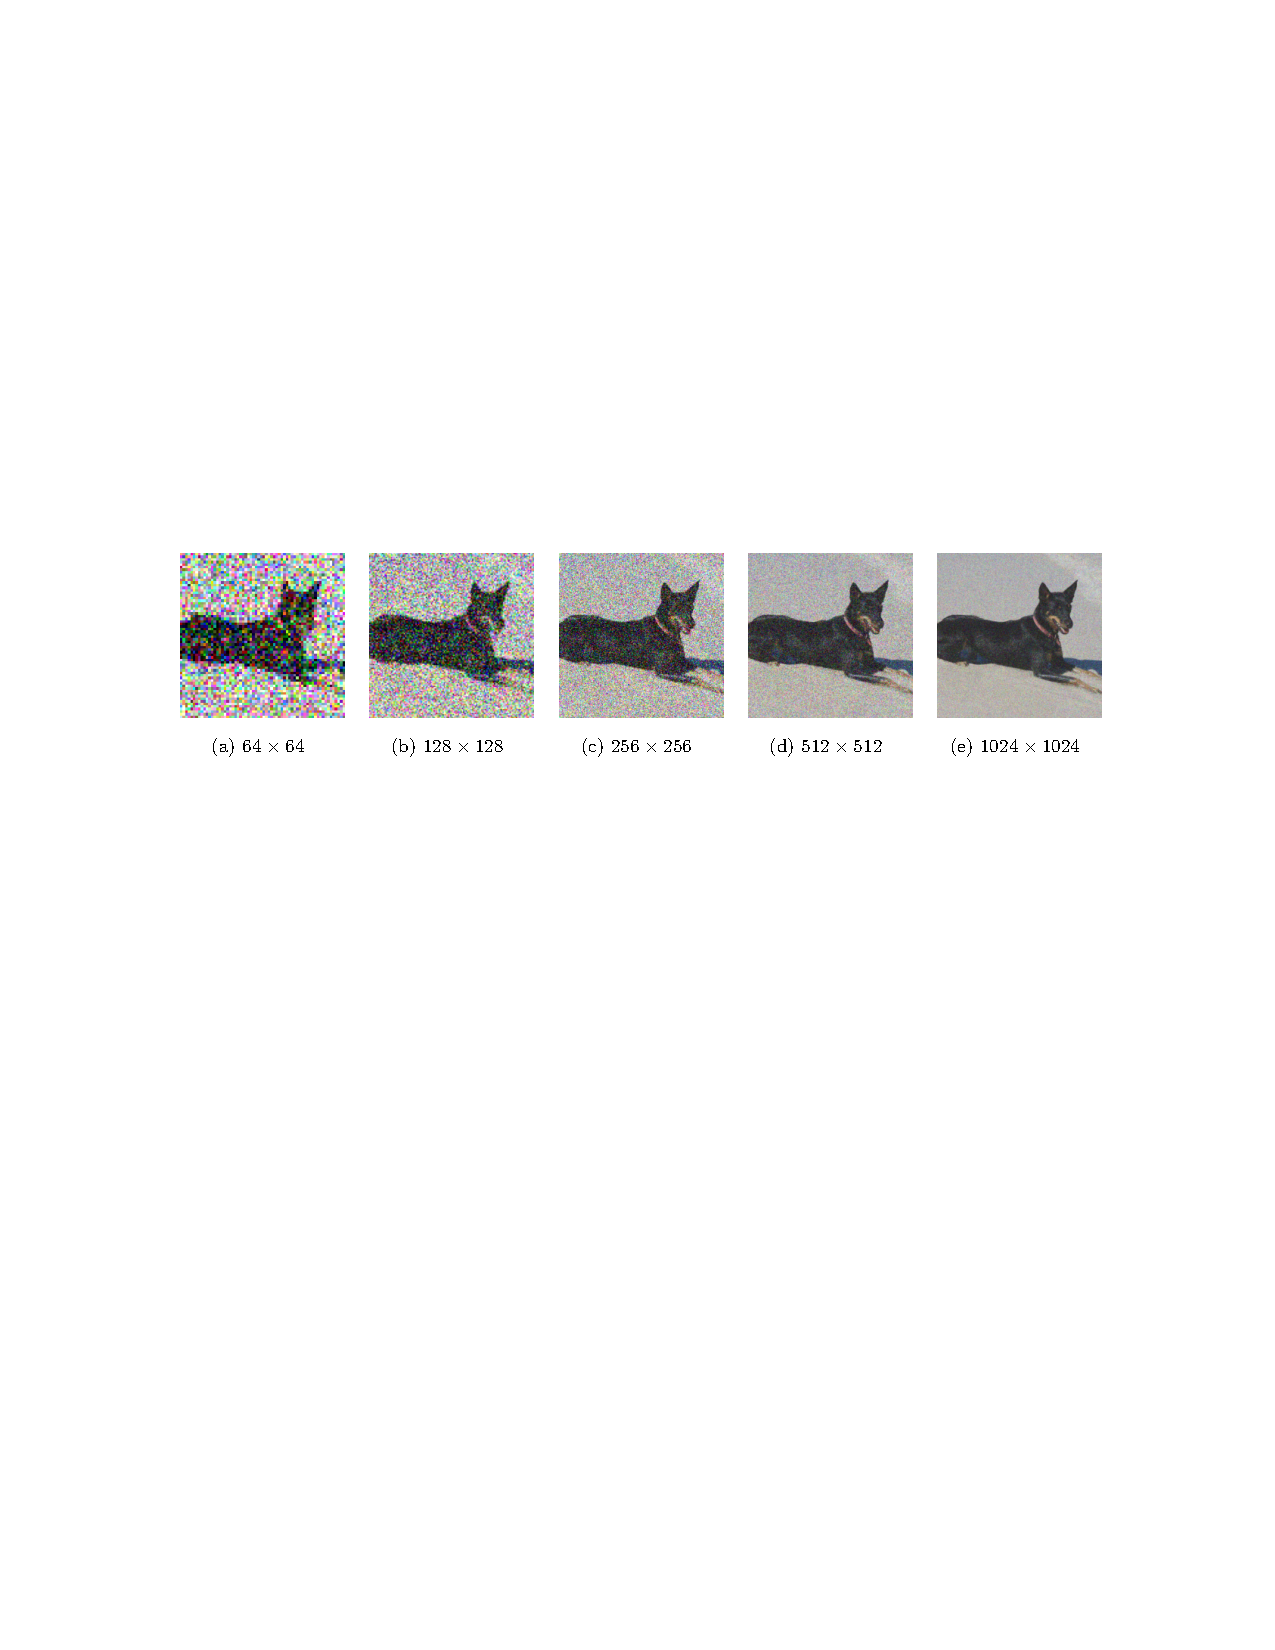
\includegraphics[width=0.8\textwidth]{images/dm/noise_resolution}
            \caption{Imágenes obtenidas desde \cite{nichol2021improved} y \cite{chen2023importancenoiseschedulingdiffusion}.}
        \end{figure}
    }
    \only<2>{
        \insertimage{dm/cyclegan}{1}{Imagen obtenida desde \cite{zhu2020unpairedimagetoimagetranslationusing}.}
    }
    \only<3>{
        \insertimage{dm/short_time}{1}{Imagen obtenida desde \cite{debortoli2023diffusionschrodingerbridgeapplications}.}
    }
\end{frame}

\section{Problema de Schrödinger}

\begin{frame}{Problema de Schrödinger | Formulación dinámica}
    \uncover<1->{
        Considerando $\xspace,\yspace\subset\R^d$, el siguiente problema generativo corrige las limitaciones mencionadas:
        \begin{block}{SBP (formulación dinámica)}
            El puente de Schrödinger entre dos medidas $\mu\in\probmeasure{\xspace}$ y $\nu\in\probmeasure{\yspace}$ es el (único) proceso estocástico que resuelve el problema
            \begin{equation*}
                \min_{P\,:\,(P_0\sim\mu) \wedge (P_1\sim\nu)} \KL{P}{R},
            \end{equation*}
            \begin{equation*}
                \text{donde }\begin{cases}
                    R\text{ es la ley de } x_t = f(x_t,t)\d t + g(t)\d w_t \\
                    P\text{ es la ley de } x_t = \left[f(x_t,t)+\fcolor{v(x_t,t)}\right]\d t + g(t)\d w_t
                \end{cases}
            \end{equation*}
        \end{block}
    }
    \uncover<2>{
        Por simplicidad, se considerará siempre que $R$ es el movimiento browiano con difusividad $\sigma>0$ (i.e., $f\equiv 0$ y $g(t)=\sigma$).
    }
\end{frame}

\begin{frame}{Problema de Schrödinger | Formulación dinámica}
    \only<1>{
        \insertimage{eot_sbp/sbp1}{1}{Puentes de Schrödinger para $\sigma=1$.}
    }
    \only<2>{
        \insertimage{eot_sbp/sbp0.1}{1}{Puentes de Schrödinger para $\sigma=0.1$.}
    }
    \only<3>{
        \insertimage{eot_sbp/sbp0.05}{1}{Puentes de Schrödinger para $\sigma=0.05$.}
    }
\end{frame}

\begin{frame}{Problema de Schrödinger | Formulación estática}
    \uncover<1->{
        Se puede demostrar la siguiente descomposición:
        \begin{equation*}
            \KL{P}{R} = \KL{P_{01}}{R_{01}} + \E{(x,y)\sim P_{01}}{\KL{P_{|xy}}{R_{|xy}}}.
        \end{equation*}
    }
    \uncover<2->{
        Por lo tanto, el SBP dinámico se puede reducir a un problema estático enfocado únicamente en los extremos del proceso:
        \begin{equation*}
            \underbrace{\min_{P\,:\,(P_0\sim\mu) \wedge (P_1\sim\nu)} \KL{\fcolor{P}}{R}}_{\text{problema dinámico}} = \underbrace{\min_{P_{01}\in\Pi(\mu,\nu)} \KL{\fcolor{P_{01}}}{R_{01}}}_{\text{problema estático}},
        \end{equation*}
        donde $\Pi(\mu,\nu) := \{\pi\in\probmeasure{\xspace\times\yspace}\,: (\pi_0\sim\mu) \wedge (\pi_1\sim\nu)\}$.
    }

    \uncover<3>{
        Si $P_{01}^*$ es la (única) solución del SBP estático, la (única) solución del SBP dinámico es
        \begin{equation*}
            P^*(\cdot) = \int_{\xspace\times\yspace} R_{|xy}(\cdot) \d P_{01}^*(x,y).
        \end{equation*}
    }
\end{frame}

\begin{frame}{Problema de Schrödinger | Formulación estática}
    \begin{center}
        \only<1>{
            \insertimage{eot_sbp/static1}{0.7}{Plan de transporte para $\sigma=1$.}
        }
        \only<2>{
            \insertimage{eot_sbp/static0.1}{0.7}{Plan de transporte para $\sigma=0.1$.}
        }
        \only<3>{
            \insertimage{eot_sbp/static0.01}{0.7}{Plan de transporte para $\sigma=0.01$.}
        }
        \only<4>{
            \insertimage{eot_sbp/static0.005}{0.7}{Plan de transporte para $\sigma=0.005$.}
        }
    \end{center}
\end{frame}

\begin{frame}{Problema de Schrödinger | Formulación estática}
    \uncover<1,2>{
        El SBP estático es equivalente al problema de transporte óptimo con regularización entrópica (EOT).
    }
    \uncover<2>{
        \begin{align*}
             & \KL{P_{01}}{R_{01}}                                                                                                                                                                                                         \\
             & \quad = \frac{1}{\sigma}\rparent{\underbrace{\int_{\xspace\times\yspace} \frac{1}{2} \norm{x-y}^2 \d P_{01}(x,y)}_{\text{costo de transporte}} + \underbrace{- \sigma\cdot\entropy{P_{01}}}_{\text{regularizador}}} + \cte,
        \end{align*}

        donde $\entropy{P_{01}}$ es la entropía (diferencial) de $P_{01}$.
    }

    \uncover<3>{
        En general, todo SBP (con una cierta medida de referencia) puede ser transformado a un problema de EOT (con una cierta función de costo), y viceversa.
    }

\end{frame}

\section{Transporte óptimo}

\begin{frame}{Transporte óptimo | Problema de Kantorovich}
    \uncover<1->{
        \begin{block}{Problema de Kantorovich}
            Si $c:\xspace\times\yspace\to\R$ es una medida de discrepancia, el problema de Kantorovich entre $\mu\in\probmeasure{\xspace}$ y $\nu\in\probmeasure{\yspace}$ es:
            \begin{equation*}
                \min_{\pi \in \Pi(\mu,\nu)} \int_{\xspace\times\yspace} c(x,y) \d\pi(x, y).
            \end{equation*}
        \end{block}
    }
    \begin{itemize}
        \item<2> Bajo ciertas condiciones, el problema de Kantorovich tiene solución.
        \item<3> Este funcional de costo, más un término regularizador, equivale al SBP estático.
        \item<4> Por simplicidad, se considerará siempre que $c(x,y)=\frac{1}{2}\norm{x-y}^2$.
    \end{itemize}
\end{frame}

\begin{frame}{Transporte óptimo | Problema de Kantorovich}
    El problema de Kantorovich discreto es un problema lineal, por lo que se puede resolver eficientemente.
    \begin{columns}
        \begin{column}{0.49\textwidth}
            \insertimage{ot/kantorovich_discrete_solution}{1}{Caso discreto.}
        \end{column}
        \begin{column}{0.49\textwidth}
            \insertimage{ot/kantorovich_continuous_solution}{1}{Caso continuo discretizado.}
        \end{column}
    \end{columns}
\end{frame}

\begin{frame}{Transporte óptimo | Distancia de Wasserstein}
    \uncover<1>{
        El problema de Kantorovich induce una métrica en (un subconjunto de) $\probmeasure{\xspace}$, llamada distancia de Wasserstein. Para $p\in[1,\infty]$:
        \begin{equation*}
            \wasserstein{p}{\mu,\nu}^p := \min_{\pi\in\Pi(\mu,\nu)}\int_{\xspace\times\yspace} \norm{x-y}^p\d\pi(x,y)
        \end{equation*}
    }
    \only<2>{
        Es posible interpolar entre dos distribuciones de probabilidad a través de una \textit{curva} de distribuciones en $\probmeasure{\xspace}$.
        \insertimage{eot_sbp/mixture}{0.8}{Interpolación entre dos distribuciones gaussianas.}
    }
\end{frame}

\begin{frame}{Transporte óptimo | Distancia de Wasserstein}
    La distancia de Wasserstein tiene buenas propiedades.
    \begin{itemize}
        \item<2> Es una distancia completa.
        \item<3> Es más débil que la distancia en variación total.
        \item<4> Más aún, metriza la convergencia débil de medidas.
        \item<5> Puede ser optimizada por redes neuronales:
              si $g_\theta(z)\sim\mu_\theta$ es un modelo generativo neuronal de variable latente $z\sim\gaussian{0}{\identity{l}}$,  entonces $\theta\mapsto\wasserstein{1}{\mu_\theta,\mu_{\text{true}}}$ es diferenciable.
    \end{itemize}
    \uncover<6>{
        Todas estas propiedades motivan a usar la distancia de Wasserstein en modelos generativos entrenados con redes neuronales.
    }
\end{frame}

\begin{frame}{Transporte óptimo | Regularización}
    El problema de Kantorovich es costoso de resolver, por lo que se preferirá una versión regularizada:
    \begin{block}{EOT (a.k.a. SBP estático)}
        El problema de Kantorovich regularizado es
        \begin{equation*}
            \min_{\pi\in\Pi(\mu,\nu)} \int_{\xspace\times\yspace} \norm{x-y}^2 \d\pi(x,y)\, \fcolor{-\, \sigma\,\entropy{\pi}},
        \end{equation*}
        donde $\entropy{\pi}=-\int_{\xspace\times\yspace} \log\parent{\frac{\d\pi}{\d x\text{d} y}(x,y)}\d\pi(x,y)$ es la entropía de $\pi$ y $\sigma>0$ es un ponderador de regularización.
    \end{block}
    \uncover<2>{
        Esta versión regularizada es más fácil de resolver y tiene buenas propiedades.
    }
\end{frame}

\begin{frame}{Transporte óptimo | Regularización}
    \only<1>{
        \insertimage{eot_sbp/sinkhorn1}{1}{Plan de transporte entrópico para $\sigma=1$.}
    }
    \only<2>{
        \insertimage{eot_sbp/sinkhorn0.1}{1}{Plan de transporte entrópico para $\sigma=0.1$.}
    }
    \only<3>{
        \insertimage{eot_sbp/sinkhorn0.01}{1}{Plan de transporte entrópico para $\sigma=0.01$.}
    }
    \only<4>{
        \insertimage{eot_sbp/sinkhorn0.001}{1}{Plan de transporte entrópico para $\sigma=0.001$.}
    }
    \only<5>{
        \insertimage{eot_sbp/sinkhorn0.0005}{1}{Plan de transporte entrópico para $\sigma=0.0005$.}
    }
\end{frame}

\begin{frame}{OT y SBP | Formulación dual}
    \begin{block}{OT}
        El problema dual del problema de Kantorovich es
        \begin{equation*}
            \sup_{\phi,\psi} \int_\xspace \phi(x) \d\mu(x) + \int_\yspace \psi(y) \d\nu(y)
            \quad\text{s.a } \phi(x)+\psi(y)\leq \norm{x-y}^2.
        \end{equation*}
    \end{block}
    \uncover<2>{
    \begin{block}{SBP estático}
        El problema dual del SBP estático es
        \begin{equation*}
            \sup_{\phi,\psi} \int_\xspace \phi(x) \d\mu(x) + \int_\yspace \psi(y) \d\nu(y) \fcolor{ \,-\, \sigma\int e^{\frac{\phi(x)+\psi(y)-\norm{x-y}^2}{\sigma}-1}\d\pi(x,y)}.
        \end{equation*}
        Además, la única solución del SBP estático es
        \begin{equation*}
            \d\pi(x,y) = e^{\frac{\phi(x)+\psi(y)-\norm{x-y}^2}{\sigma}-1}\d\mu(x)\d\nu(y)
        \end{equation*}
    \end{block}
    }
\end{frame}

\begin{frame}{OT y SBP | Como problemas de control óptimo}
    \begin{block}{OT dinámico (Benamou-Brenier)}
        \begin{equation*}
            \min_{v} \E{x}{\int_0^1 \frac{1}{2}\norm{v(x_t,t)}^2 \d t}
            \quad\text{sujeto a}\quad
            \begin{cases}
                \d x_t = v(x_t,t) \d t \\
                (x_0\sim\mu) \wedge (x_1\sim\nu),
            \end{cases}
        \end{equation*}
        Se puede sustituir la ODE por su ecuación de continuidad.
    \end{block}
    \uncover<2>{
    \begin{block}{SBP dinámico}
        \begin{equation*}
            \min_{v} \E{x}{\int_0^1 \frac{1}{2}\norm{v(x_t,t)}^2 \d t}
            \quad\text{sujeto a}\quad
            \begin{cases}
                \d x_t = v(x_t,t) \d t \fcolor{\,+\, \sigma\d w_t} \\
                (x_0\sim\mu) \wedge (x_1\sim\nu),
            \end{cases}
        \end{equation*}
        Se puede sustituir la SDE por su ecuación de Fokker-Planck.
    \end{block}
    }
\end{frame}

\begin{frame}{OT y SBP | Como problemas de control óptimo}
    \insertimage{ot/distr_transform}{1}{Imagen obtenida desde \cite{albergo2023stochasticinterpolantsunifyingframework}.}
\end{frame}

\begin{frame}{OT y SBP | Como sistema de PDEs}
    \begin{itemize}
        \item<1> Se pueden sustituir las dinámicas por PDEs que las caractericen.
        \item<2> La optimalidad de los problemas de control también se puede caracterizar por PDEs.
    \end{itemize}
    \uncover<3>{
    \begin{block}{Caracterización de optimalidad para OT}
        \begin{equation*}
            \begin{cases}
                \partial_t \rho + \nabla\cdot(\rho \nabla\lambda) = 0      & \text{(eq. continuidad)} \\
                \partial_t \lambda + \frac{1}{2}\norm{\nabla\lambda}^2 = 0 & \text{(Hamilton-Jacobi)}
            \end{cases}
        \end{equation*}
    \end{block}
    }
    \uncover<4>{
    \begin{block}{Caracterización de optimalidad para SBP (sistema de Schrödinger)}
        \begin{equation*}
            \begin{cases}
                \partial_t \rho + \nabla\cdot(\rho \nabla\lambda) \fcolor{\,-\,\frac{\sigma^2}{2}\Delta\rho}= 0          & \text{(Fokker-Planck)}           \\
                \partial_t \lambda + \frac{1}{2}\norm{\nabla\lambda}^2 \fcolor{+\,\frac{\sigma^2}{2}\Delta\lambda} = 0 & \text{(Hamilton-Jacobi-Bellman)}
            \end{cases}
        \end{equation*}
    \end{block}
    }
\end{frame}

\begin{frame}{OT y SBP | Distintos modelos}
    \begin{columns}
        \begin{column}{0.7\textwidth}
            \begin{itemize}
                \item<1> Todos estas formulaciones son equivalentes entre sí.
                \item<2> Esta diversidad de formulaciones permite atacar el problema de Schrödinger desde distintos ángulos.
                \item<3> La mayoría de técnicas usadas son variantes del algoritmo de Sinkhorn.
                \item<4> Un modelo para el SBP puede, en principio, resolver los mismos problemas que un modelo de difusión.
            \end{itemize}
        \end{column}
        \begin{column}{0.29\textwidth}
            \only<4>{
                \insertimage{eot_sbp/i2sb}{1}{Imagen obtenida desde \cite{liu2023i2sbimagetoimageschrodingerbridge}.}
            }
            \only<5>{
                \insertimage{eot_sbp/lsb}{0.8}{Imagen obtenida desde \cite{korotin2024lightschrodingerbridge}.}
            }
        \end{column}
    \end{columns}
\end{frame}

\begin{frame}{Conclusión}
    \begin{itemize}
        \item<1> El problema de Schrödinger puede verse como un paradigma generativo que generaliza los modelos de difusión.
        \item<2> Este modelo es complejo de formular dado que ha sido estudiado principalmente desde una perspectiva matemática.
        \item<3> En consecuencia, en este trabajo se buscó una presentación sencilla de las cosas más importantes, con demostraciones simples e implementaciones minimales.
        \item<4> No obstante, se intentó mantener siempre la coherencia matemática, la cual muchas veces es, o bien escasa, o bien engorrosa en la formulación.
        \item<5> Se espera que este trabajo pueda servir como punto de introducción a cualquier persona interesada en el problema de Schrödinger desde una perspectiva del aprendizaje automático.
    \end{itemize}
\end{frame}

\begin{frame}
    \centering
    \Large{El Problema del Puente de Schrödinger como Generalización de los Modelos de Difusión}
\end{frame}

\end{document}